\section{MS COCO}
The MS COCO dataset \parencite{chen2015microsoft} contains 12 superordinate categories which contain 80 basic-level categories. Table \ref{tab:app_coco_categories} presents the mappings of the categories as well as the occurrence counts in the train split of the dataset. 

\begin{table}[]
	\begin{tabularx}{\linewidth}{|X|X|l|}
		\hline
		\textbf{Superordinate category}                                    & \textbf{Basic-level categories} & \textbf{Counts}  \\ \hline
		Person & person & 42,151\\  \hline
		accessory & backpack, umbrella, andbag, tie, suitcase &11,172 \\  \hline
		indoor & book, clovk, vase, scissors, teddy bear, hair drier, toothbrush & 9,308\\  \hline
		appliance & microwave, oven, toaster, sink, refrigerator & 4,494 \\  \hline
		food & banana, apple, sandwich, orange, broccoli, carrot, hot dog, pizza, donut, cake & 9,740 \\  \hline
		kitchen & bottle, wine glass, cup, fork, knife, spoon, bowl & 11,226\\  \hline
		sports & frisbee, skis, snowboard, sports ball, kite, baseball bat, baseball glove, skateboard, surfboard, tennis racket &16,240 \\  \hline
		furniture & chair, couch, potted plant, bed, dining table, toilet & 17077\\  \hline
		outdoor & traffic light, fire hydrant, stop sign, parking meter, bench & 8,455\\  \hline
		animal & bird, cat, dog, horse, sheep, cow, elephant, bear, zebra, giraffe & 16,352\\  \hline
		electronic & TV, laptop, mouse, remote, keyboard, cell phone & 7,507 \\  \hline
		vehicle & bicycle, car, motorcycle, airplane, bus, train, truck, boat & 18,547\\ 
		\hline
	\end{tabularx}
	\caption{\label{tab:app_coco_categories} MS COCO basic-level object categories mapped to their superordinate categories, along with counts of the superordinate categories in the train split.}
\end{table}

\section{REINFORCE Pseudo-algorithm}
\pt{TODO}

\section{Speaker Architecture Grid Search}
\label{app:grid_search}

For conducting the experiments in this thesis, different hyperparameters of the reference game were explored in a grid search prior to completing the main experiments. The following hyperparameters were considered: the structural loss weight $\lambda_s \in \{0, 0.5, 0.75, 1\}$, the decoding strategy (exponential, greedy, pure, top-k) and different pretrained speakers. Additionally, different structural loss calculations were considered (see below for details). 

Due to computational constraints, not the full space of configurations was explored, but rather representative experiments in this space were conducted. The grid searches proceeded by training the speaker and listener agent with given configurations for one epoch on a reference game on 15,000 images. 

The first grid search over decoding strategies and structural loss weight, given a teacher-forcing only pretrained speaker revealed that a minimal structural weight of 0.75 was necessary for a reference game with pure decoding with above chance performance (Fig. \ref{fig:coco_grid_Ls_decoding_TF_only}). For greedy decoding, the reference games were successful for all weight configurations. The only correctly implemented exponential decoding experiments were conducted with the structural weights 0.75 and 1, and did not show qualitative improvements compared to pure decoding, so this decoding strategy was left out of further experiments. Furthermore, these results indicated that pure decoding based sampling made the policy learning more difficult for the speaker compared to greedy decoding, as can be observed from the magnitude and variance of the speaker loss for $\lambda_s = 0$ (which amounts to functional-only learning; Fig. \ref{fig:coco_grid_Ls_decoding_TF_only}, upper left).

\begin{figure}[h]
	\centering
	\includegraphics[width=\linewidth]{images/grid_search_TF_only_Ls_decoding.png}
	\caption{Grid search results over different $\lambda_s$ weights (columns) and decoding strategies during a reference game. Upper row shows total speaker train losses, bottom row shows listener train accuracies. Note the different y-axis scales of the last two plots in the upper row.}
	\label{fig:coco_grid_Ls_decoding_TF_only}
\end{figure}

The second grid search was conducted over different speaker pretraining strategies, testing the different speakers in reference games with pure and greedy decoding, and structural weights of 0 and 0.75. Speakers pretrained with the following approaches were considered: teacher forcing only pretraining (see Section \ref{model_pretraining} for details on the pretraining modes), constant 0.5 rate teacher forcing with pure auto-regressive decoding, adaptive teacher forcing rate ($0.5^{epoch}$, pure auto-regressive decoding), scheduled sampling (\cite{bengio2015scheduled}, with pure or exponential decoding, k = 30 and k = 150 for the inverse sigmoid teacher forcing rate decay) and auto-regression only pretraining with top-k sampling with a temperature of 2 \parencite[following][]{lazaridou2020multi}.
Based on manual inspection, the constant 0.5 teacher-forcing rate speaker was found to be more susceptible to repeating words during generation compared to the adaptive rate speaker, so that it was left out of further experiments. Similarly, the scheduled speaker was found to generate poor captions (as measured by image captioning metrics, see Tab. \ref{coco_grid_searches_speaker_pretrain}), so it was not used in reference game experiments. 
Therefore, the adaptive rate and the top-k speakers were compared in the grid search (Fig. \ref{fig:coco_grid_pretraining_decoding}). 
They successfully played the reference game with the structural loss weight 0.75, greedy decoding configurations slightly outperforming pure decoding for both speakers. The performance of both speakers is comparable to the respective performance of the teacher-forced only speaker (Fig. \ref{fig:coco_grid_Ls_decoding_TF_only}, third column). However, very high validation perplexities in auto-regressive mode were observed for the teacher-forced speaker, but not the adaptive  and top-k speakers (Tab. \ref{coco_grid_searches_speaker_pretrain}, last row). Auto-regressive decoding is equivalent to sampling a caption and is at the core of the reference game, and is a more cognitively plausible representation of a message generation process. Therefore, the adaptive speaker was chosen for the final experiments, as it slightly outperformed the top-k speaker across decoding strategies. Noteworthily, using a speaker pretrained with both teacher forcing and auto-regression comes at a cost of somewhat decreasing the image caption quality (see Tab. \ref{coco_grid_searches_speaker_pretrain}).
Because considering different message options, as opposed to a single maximum probability token, is intuitively more plausible, pure decoding is considered as the main decoding strategy in the final experiments.\footnote{A more precise investigation of plausibly narrowing down the considered space of token from the entire vocabulary is left for future work} Top-k decoding was also explored as the decoding strategy in reference games, but those experiments did not yield above chance listener performance, so the strategy was not further pursued and these results are omitted.

\begin{figure}[h]
	\centering
	\includegraphics[width=\linewidth]{images/grid_search_pretraining_Ls_decoding.png}
	\caption{Grid search results over different pretrained speaker models, used with different decoding and $\lambda_s$ weights in a reference game. Upper row shows total speaker training losses, lower row shows listener train accuracies. Left column shows functional only training, right column shows the baseline compound training setting. ``TF'' stands for teacher forcing, ``Top-K'' stands for a speaker pretrained with top-k sampling based auto-regression only.}
	\label{fig:coco_grid_pretraining_decoding}
\end{figure}

% Please add the following required packages to your document preamble:
% \usepackage[table,xcdraw]{xcolor}
% If you use beamer only pass "xcolor=table" option, i.e. \documentclass[xcolor=table]{beamer}
\begin{table}[]
	\begin{tabularx}{\textwidth}{|l|ll|ll|ll|}
		\hline
		\textbf{Metric} & \multicolumn{2}{l|}{\textbf{TF only}}   & \multicolumn{2}{X|}{\textbf{$0.5^{epoch}$ TF rate\newline(pure decoding)}} & \multicolumn{2}{l|}{\textbf{Scheduled}} \\ \hline
		Decoding& \multicolumn{1}{l|}{greedy}  & pure     & \multicolumn{1}{l|}{greedy}                       & pure                        & \multicolumn{1}{l|}{greedy}   & pure    \\ \hline
		B-1             & \multicolumn{1}{l|}{0.649}   & 0.465    & \multicolumn{1}{l|}{0.453}                        & 0.446                       & \multicolumn{1}{l|}{0.112}    & 0.318   \\ \hline
		B-2             & \multicolumn{1}{l|}{0.469}   & 0.264    & \multicolumn{1}{l|}{0.294}                        & 0.178                       & \multicolumn{1}{l|}{0.055}    & 0.110   \\ \hline
		B-3             & \multicolumn{1}{l|}{0.324}   & 0.146    & \multicolumn{1}{l|}{0.182}                        & 0.063                       & \multicolumn{1}{l|}{0.023}    & 0.031   \\ \hline
		B-4             & \multicolumn{1}{l|}{0.222}   & 0.080    & \multicolumn{1}{l|}{0.111}                        & 0.023                       & \multicolumn{1}{l|}{0.008}    & 0.008   \\ \hline
		M               & \multicolumn{1}{l|}{0.207}   & 0.142    & \multicolumn{1}{l|}{0.155}                        & 0.126                       & \multicolumn{1}{l|}{0.062}    & 0.093   \\ \hline
		C               & \multicolumn{1}{l|}{0.666}   & 0.294    & \multicolumn{1}{l|}{0.407}                        & 0.220                       & \multicolumn{1}{l|}{0.098}    & 0.133   \\ \hline
		PPL  & \multicolumn{1}{l|}{7924.05} & 11054.95 & \multicolumn{1}{l|}{108.06}                       & 84.86                       & \multicolumn{1}{l|}{103.74}   & 110.69  \\ \hline
		
	\end{tabularx}
\caption{\label{coco_grid_searches_speaker_pretrain}Evaluation results of speaker pretraining on MS COCO with different decoding strategies during pretraining, and different testing decoding strategies. Both standard image captioning metrics and the validation caption perplexity (PPL) are reported. ``TF'' stands for teacher forcing. Scheduled sampling with pure decoding and k=150 is reported.}
\end{table}

Finally, different structural loss calculations in the reference game were considered. More specifically, a supervised calculation, i.e., a teacher forced prediction  based loss computation (``ground truth maximization'' approach)  was compared to the computation of the loss based on the auto-regressively generated caption (with pure decoding). These were compared for the teacher-forced only pretraining speaker and the adaptive speaker, with a structural loss weight of 0.75.
It was found that there only was a difference in performance when the auto-regressive generation proceeded with pure decoding, but not with greedy decoding, therefore, only the pure decoding comparison is shown in Figure \ref{fig:coco_grid_Ls_calc}. Despite the slightly better listener performance under the ground truth maximization approach (dashed lines, right plot), the auto-regressive approach was selected for the final experiments due to its plausibility for the reference game setting. That is, it is considered more plausible that the structural constraints are computed based on messages actually generated by the speaker agent as she sees fit given the image, and not on miracuolously available teacher-forced ground truth messages. 

\begin{figure}[h]
	\centering
	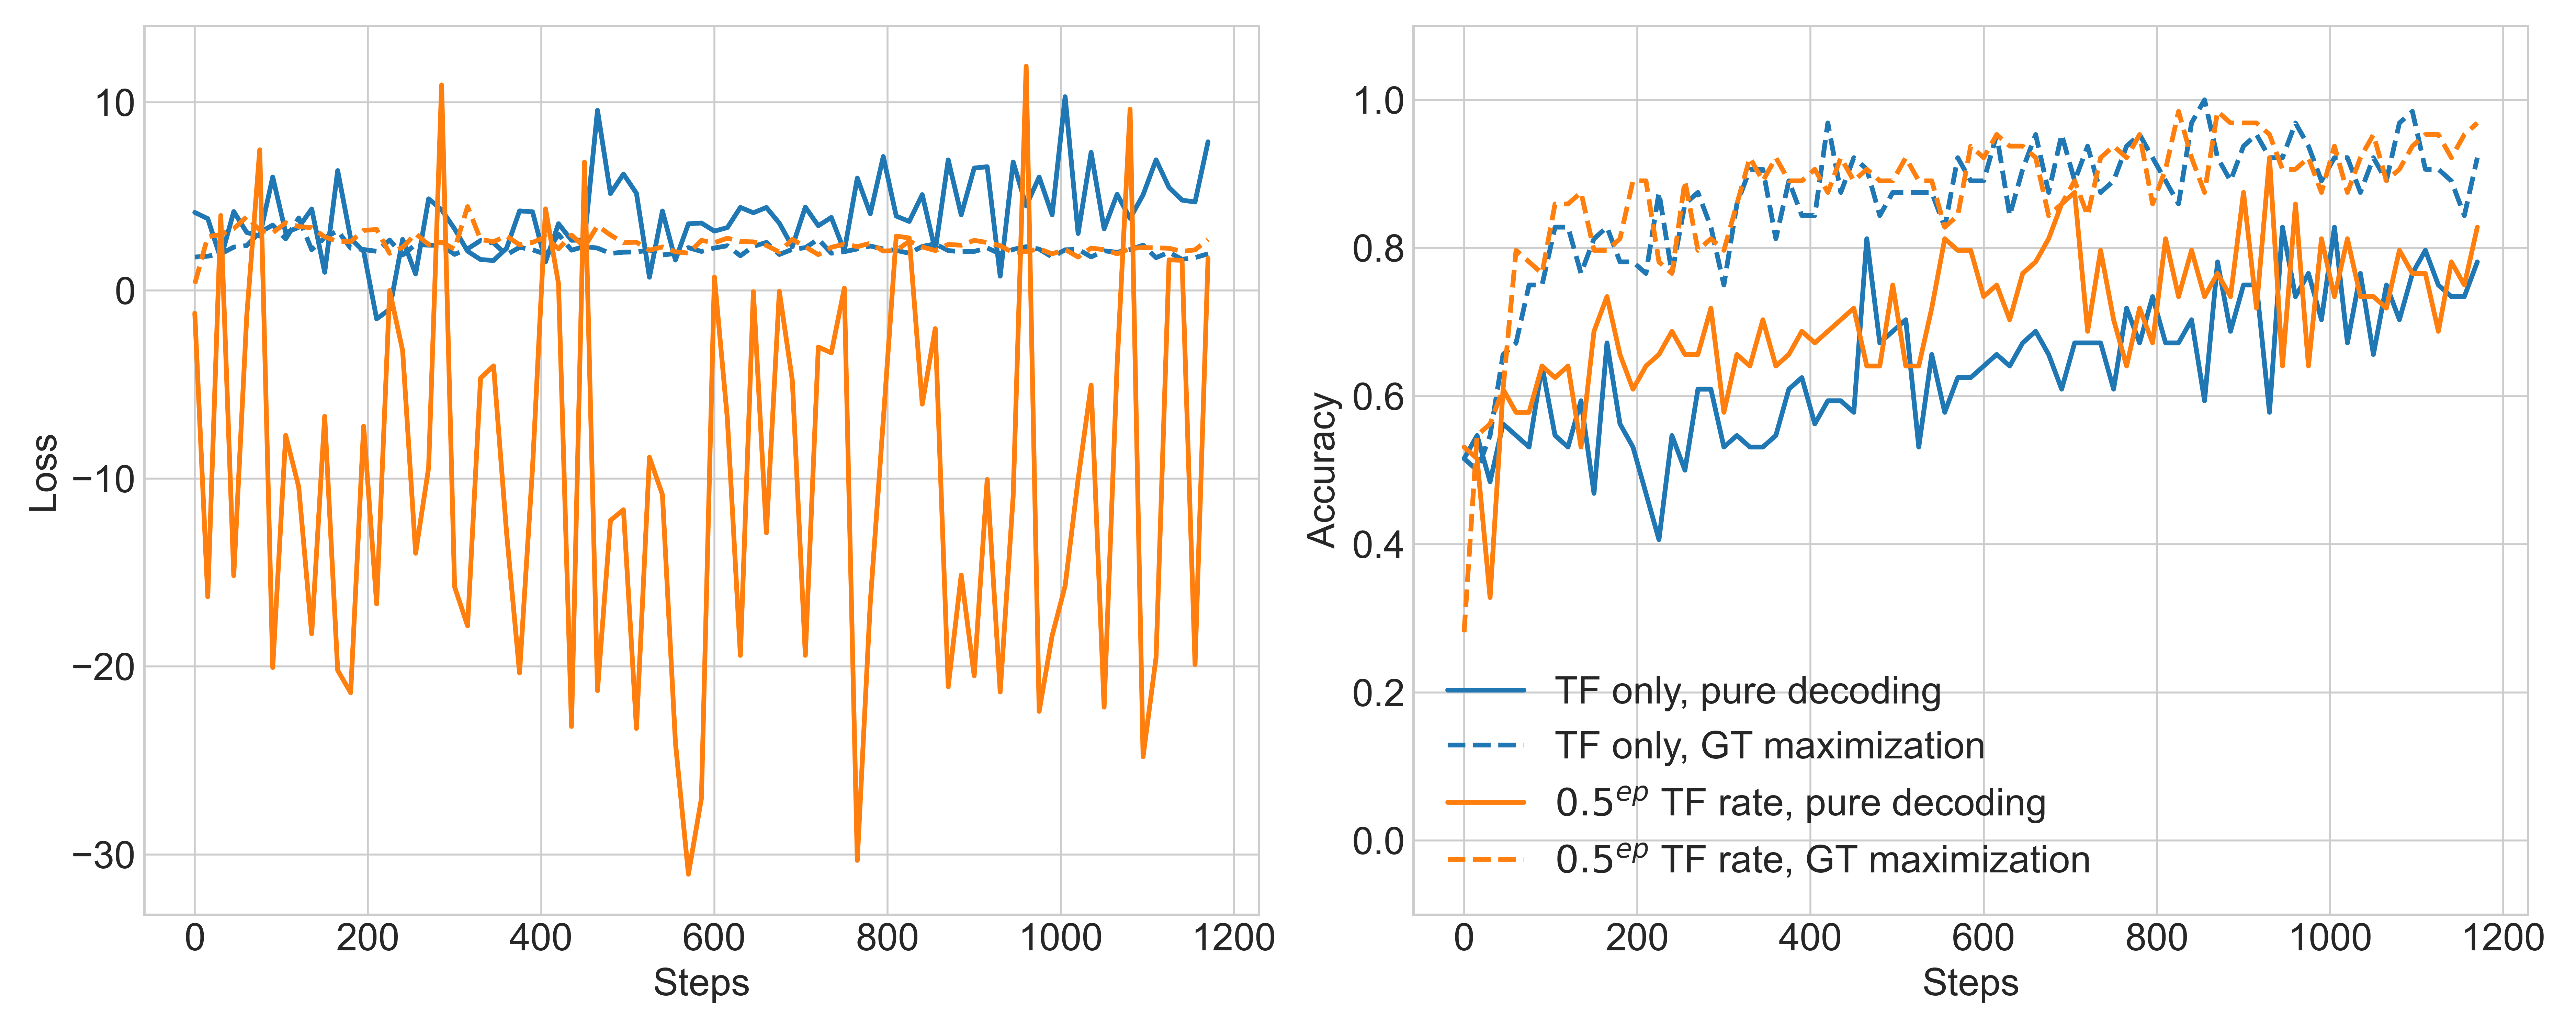
\includegraphics[width=\linewidth]{images/grid_search_Ls_calculation.png}
	\caption{Grid search results over different structural loss computation strategies in a reference game. ``TF'' stands for teacher forcing, ``GT maximization'' for supervised ground truth-based structural loss computation. Left: Total speaker training losses. Right: Listener accuracies.}
	\label{fig:coco_grid_Ls_calc}
\end{figure}

Other parameters like mean baseline subtraction in the REINFORCE update computation, different wntropy regularization weights, and adaptive learning rates for the optimizers were also explored in single experiments, but did not yield observable improvements in terms of reference game performance. Therefore, those experiments are not reported, and these configurations are not used in the final experiments.